\section{Beispiel 1: Analog Behavioral Modeling}

Zuerst wurde die Offsetspannung des Operationsverst"arkers ermittelt und mittels einer
Spannungsquelle vor dem positiven Differenzverst"arkungseingang korrigiert.

Anschlie\ss{}end wurde mittels einer AC-Analyse der Frequenzgang der Leerlaufverst"arkung ermittelt
und die Leerlaufverst"arkung sowie die Grenzfrequenzen abgelesen. Die dabei verwendete Schaltung
 ist in Abbildung \ref{fig:1_schaltung} abgebildet.
F"ur das ABM-Modell wurden dabei die ersten 2 Grenzfrequenzen ber"ucksichtigt.


Die folgenden Werte wurden abgelesen:

$A_0 = 106 dB$ \\
$f_{g1} = 24.87 Hz$ \\
$f_{g2} = 5.0871 MHz$



Das ABM-Modell wurde anschlie\ss{}end wie folgt erstellt:

\begin{verbatim}
 *-----------------------------------------------------------------------------
* connections:   non-inverting input
*                | inverting input
*                | | positive power supply
*                | | | negative power supply
*                | | | | output
*                | | | | |
.subckt MyTestOP    1 2 3 4 5
*

EFREQ 10 4 LAPLACE { V(1)-V(2) } {199526.2/(1+s/156.26) * 1/(1+s/(31963k)) }

EOUT 5 4 VALUE = { V(10)+V(4) }

.ends
*$
\end{verbatim}

Der Frequenzgang des ABM-Modells stimmte nahezu perfekt mit dem Makromodells des Operationsverst"arkers "uberein.
(siehe Abbildung \ref{fig:1_bode}

\begin{figure}%[h!]
	\centering
	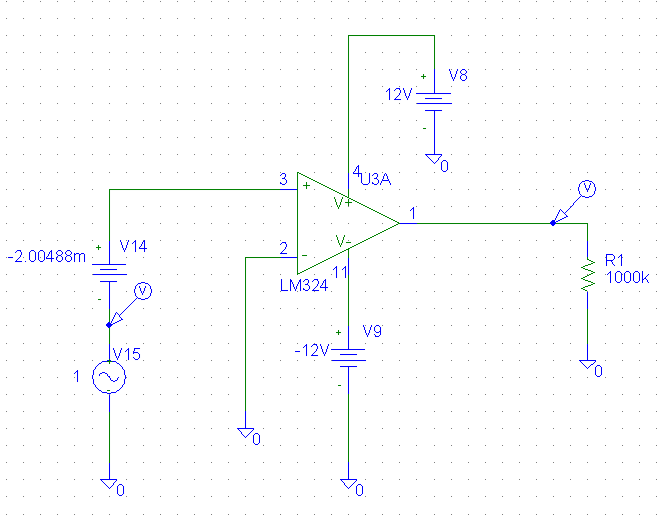
\includegraphics[width=\textwidth]{fig/1_schaltung.png}
	\caption{Schaltung zur Ermittlung des Frequenzgangs der Leerlaufverst"arkung}
	\label{fig:1_schaltung}
\end{figure}

\begin{figure}%[h!]
	\centering
	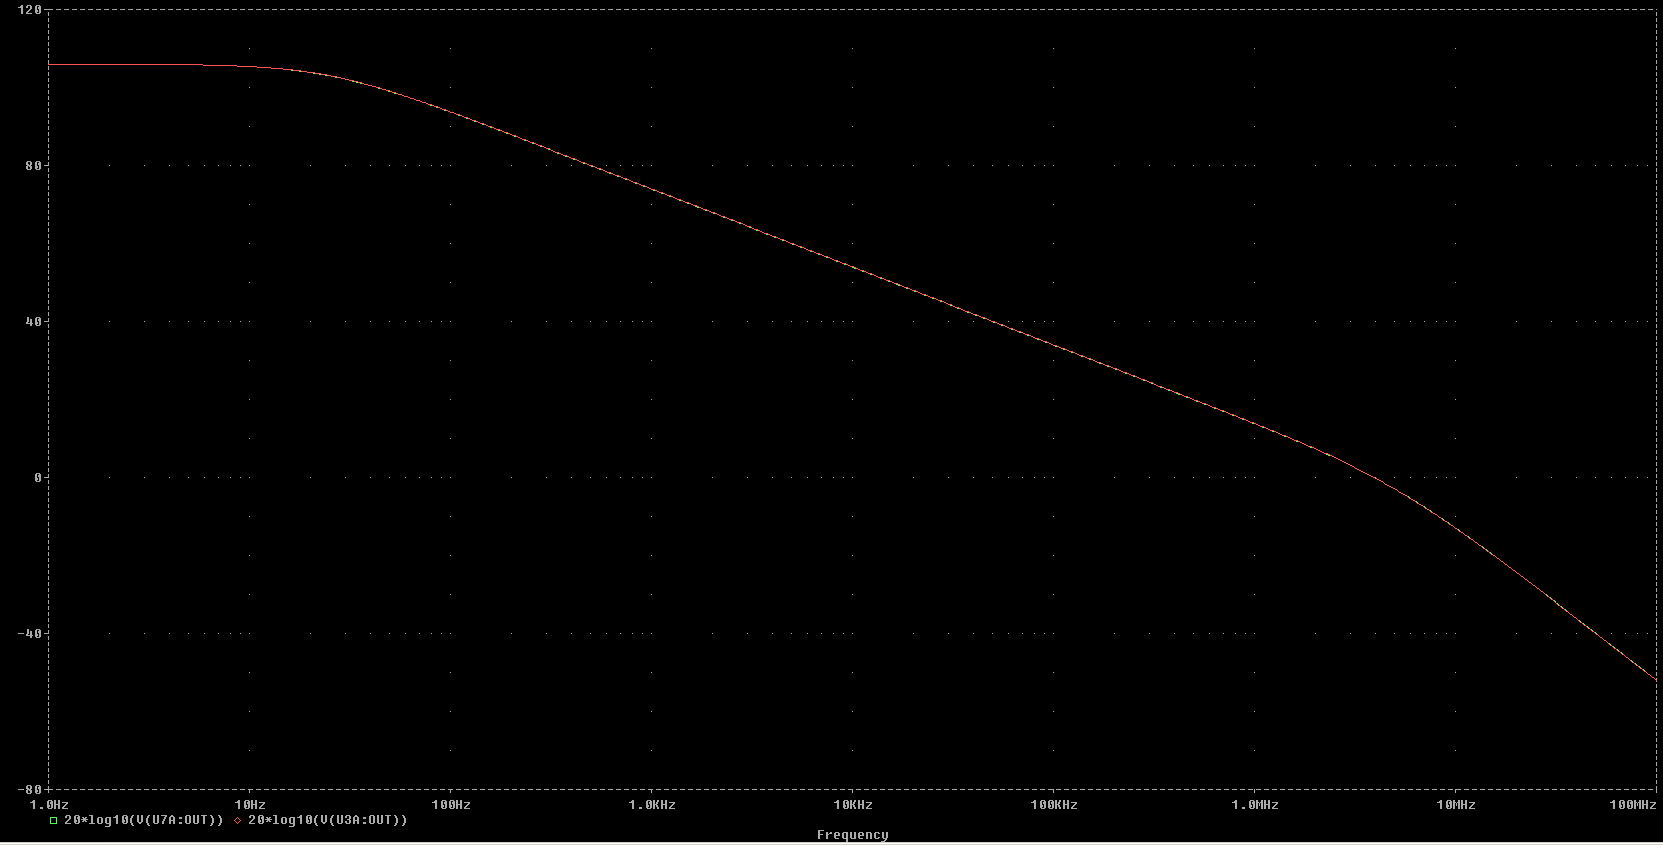
\includegraphics[width=\textwidth]{fig/1_bode.png}
	\caption{Vergleich der Bodediagramme des Makromodells und des ABM-Modells}
	\label{fig:1_bode}
\end{figure}




\section{Beispiel 2: Z"ahler}

Der Z"ahler besitzt die folgende Z"ahlabfolge:

$F_H$, $E_H$, $D_H$, $C_H$, $B_H$, $4_H$, $3_H$, $2_H$, $1_H$, $0_H$, $F_H$, ...

Die maximale Taktrate mit der die Schaltung betrieben werden kann betr"agt 16.12 MHz.

Wird diese Taktrate "uberschritten, so treten beim Timing Mode ``Maximum'' mehrere Warnungen in der Simulation auf.
Diese zeigen, dass gewisse Zeiten der Flip-Flops nicht eingehalten werden.
